%Title of section
\section{问题背景}

\begin{frame}
\frametitle{问题背景}
\begin{itemize}
    \item<1-> 虚拟机和容器
    \begin{itemize}
        \item<1-> 虚拟机:Hypervisor
        \item<1-> 容器:Namespace和Cgroups
    \end{itemize}
    \item<2-> 云计算运行模式:IaaS,PaaS和SaaS转变到CaaS
    \begin{itemize}
        \item<2-> 资源隔离
        \item<2-> 迁移开销与延迟
        \item<2-> 调度粒度
        \item<2-> 依赖距离
    \end{itemize}
    \item<3-> 能耗优化与绿色计算
\end{itemize}

\begin{figure}[htb]
\visible<1->{
    \centering
    \begin{minipage}{130pt}
    \centering
    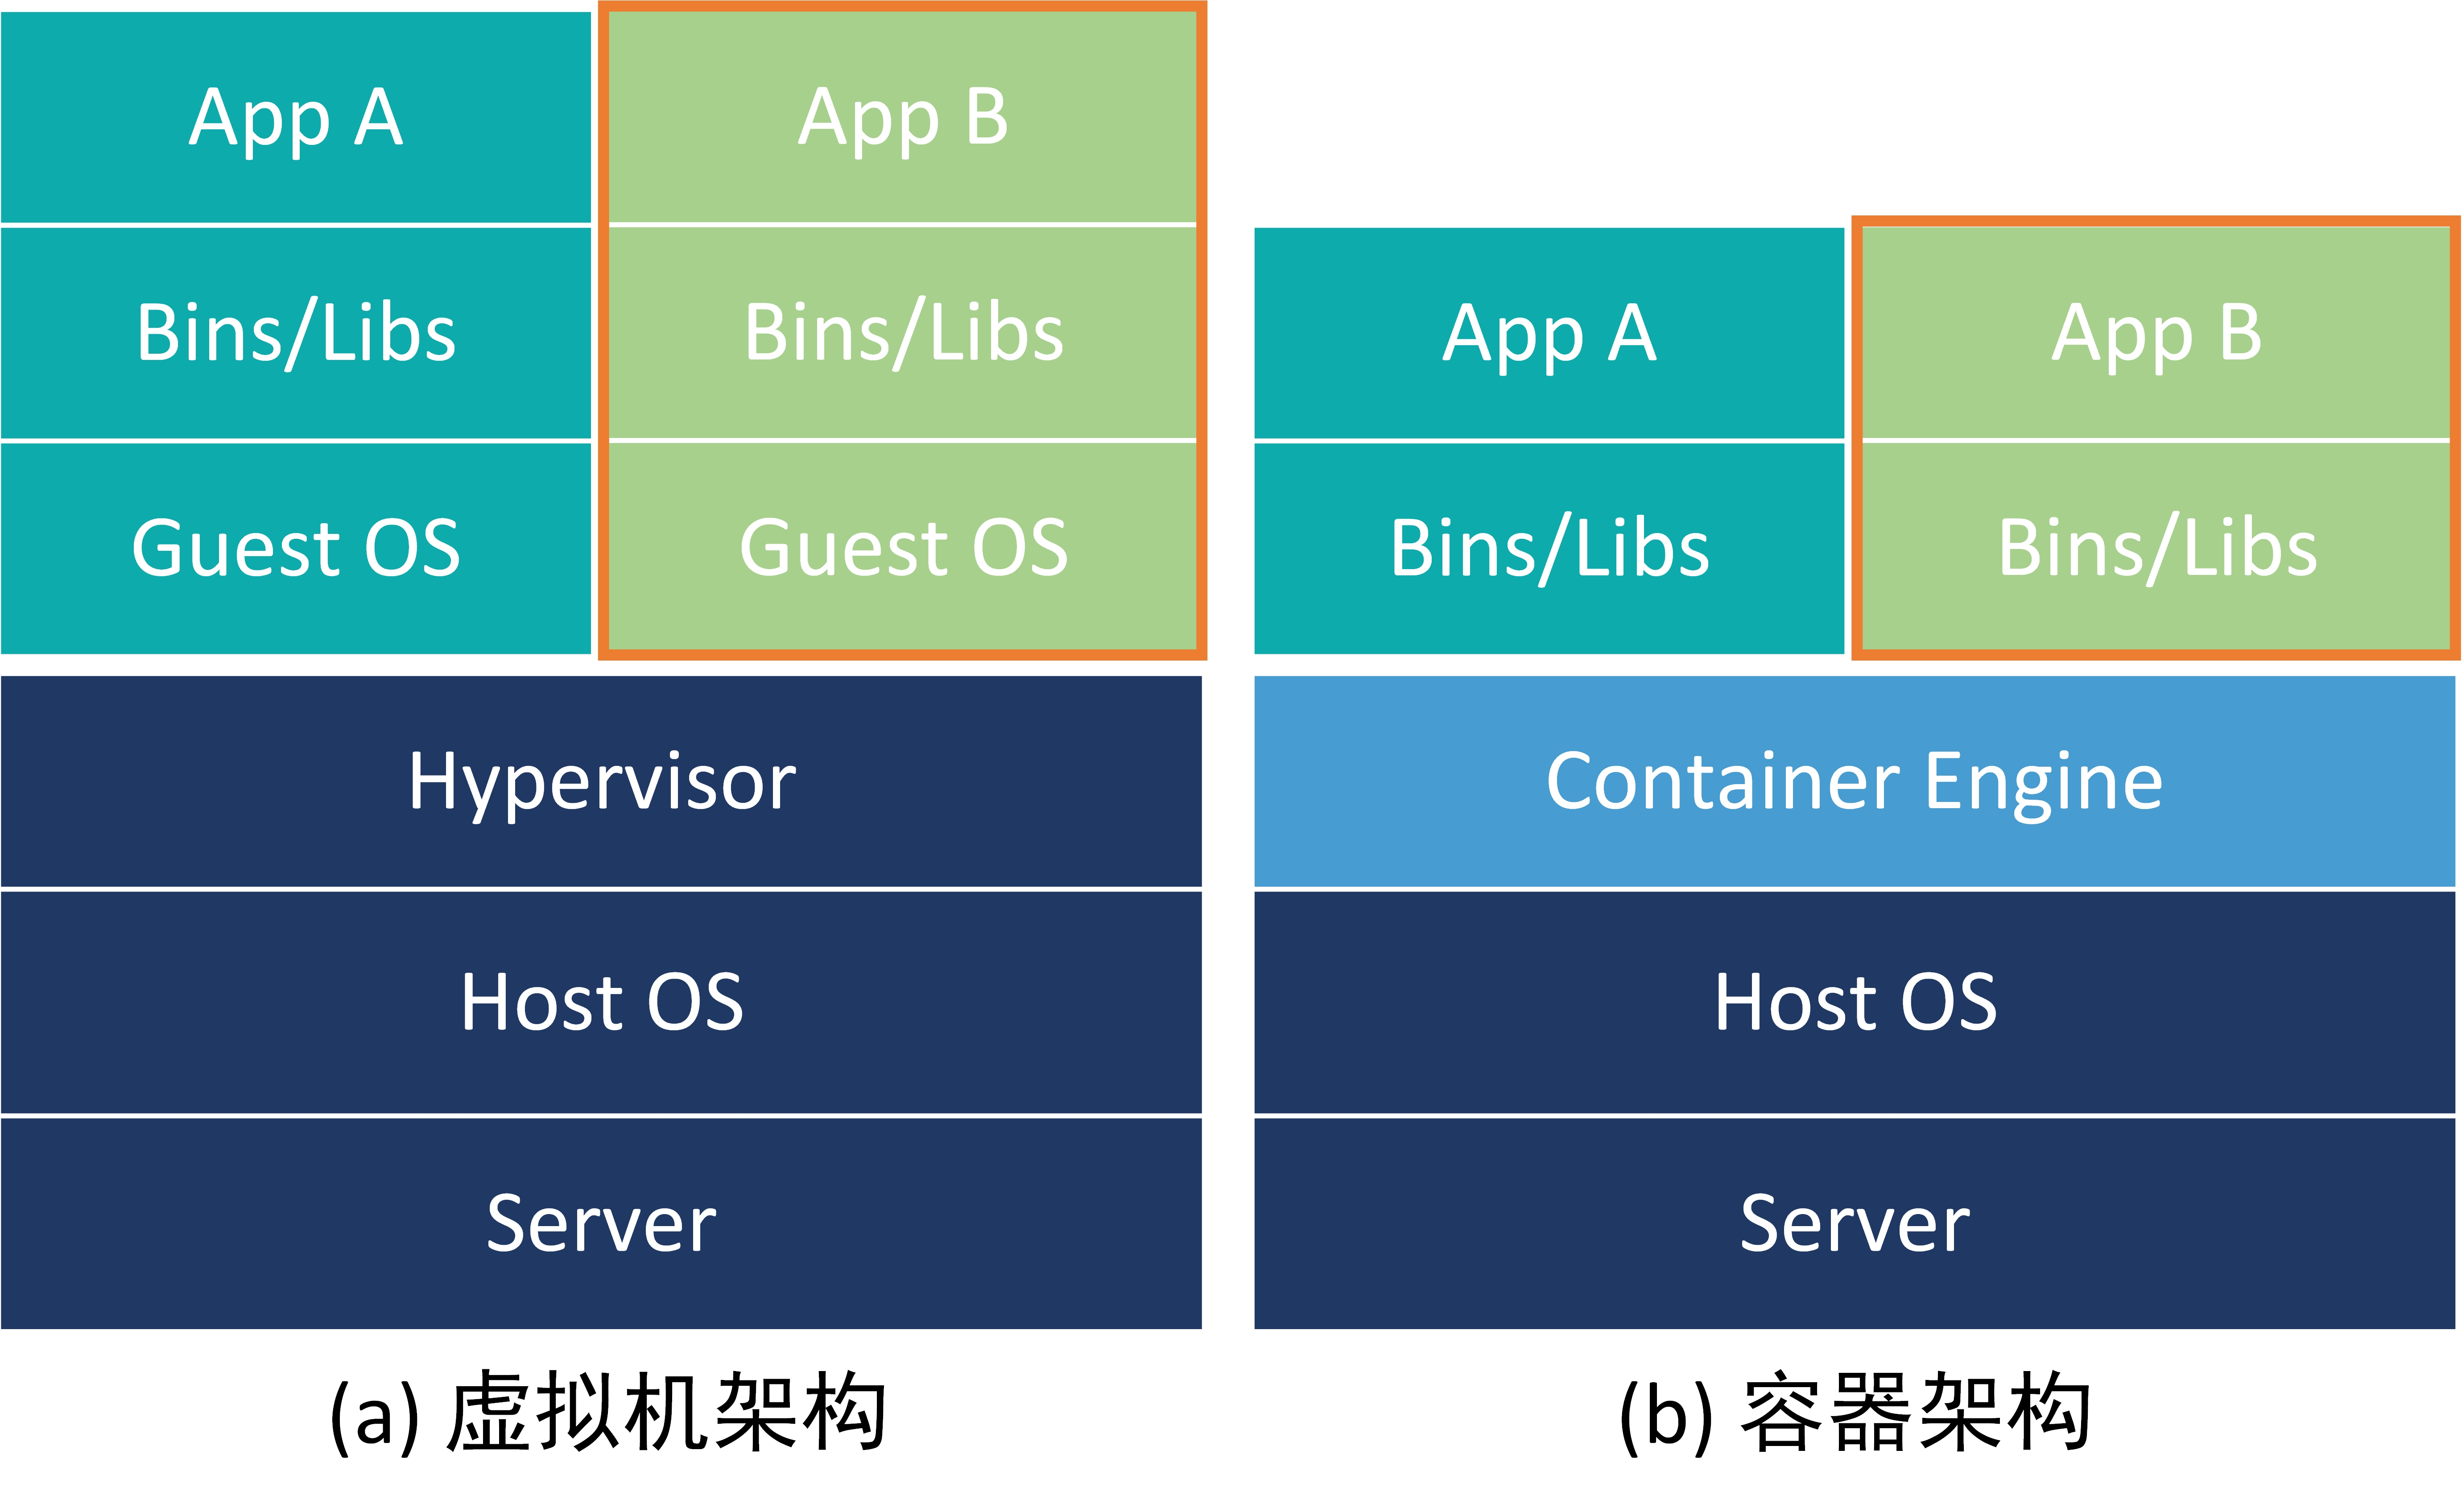
\includegraphics[scale=0.41]{figures/fig1_vm_vs_container.jpg}
    \caption{VM vs Container}
    \label{fig:fig1}
    \end{minipage}
}
\hspace{20pt}%
\visible<2->{
    \begin{minipage}{130pt}
    \centering
    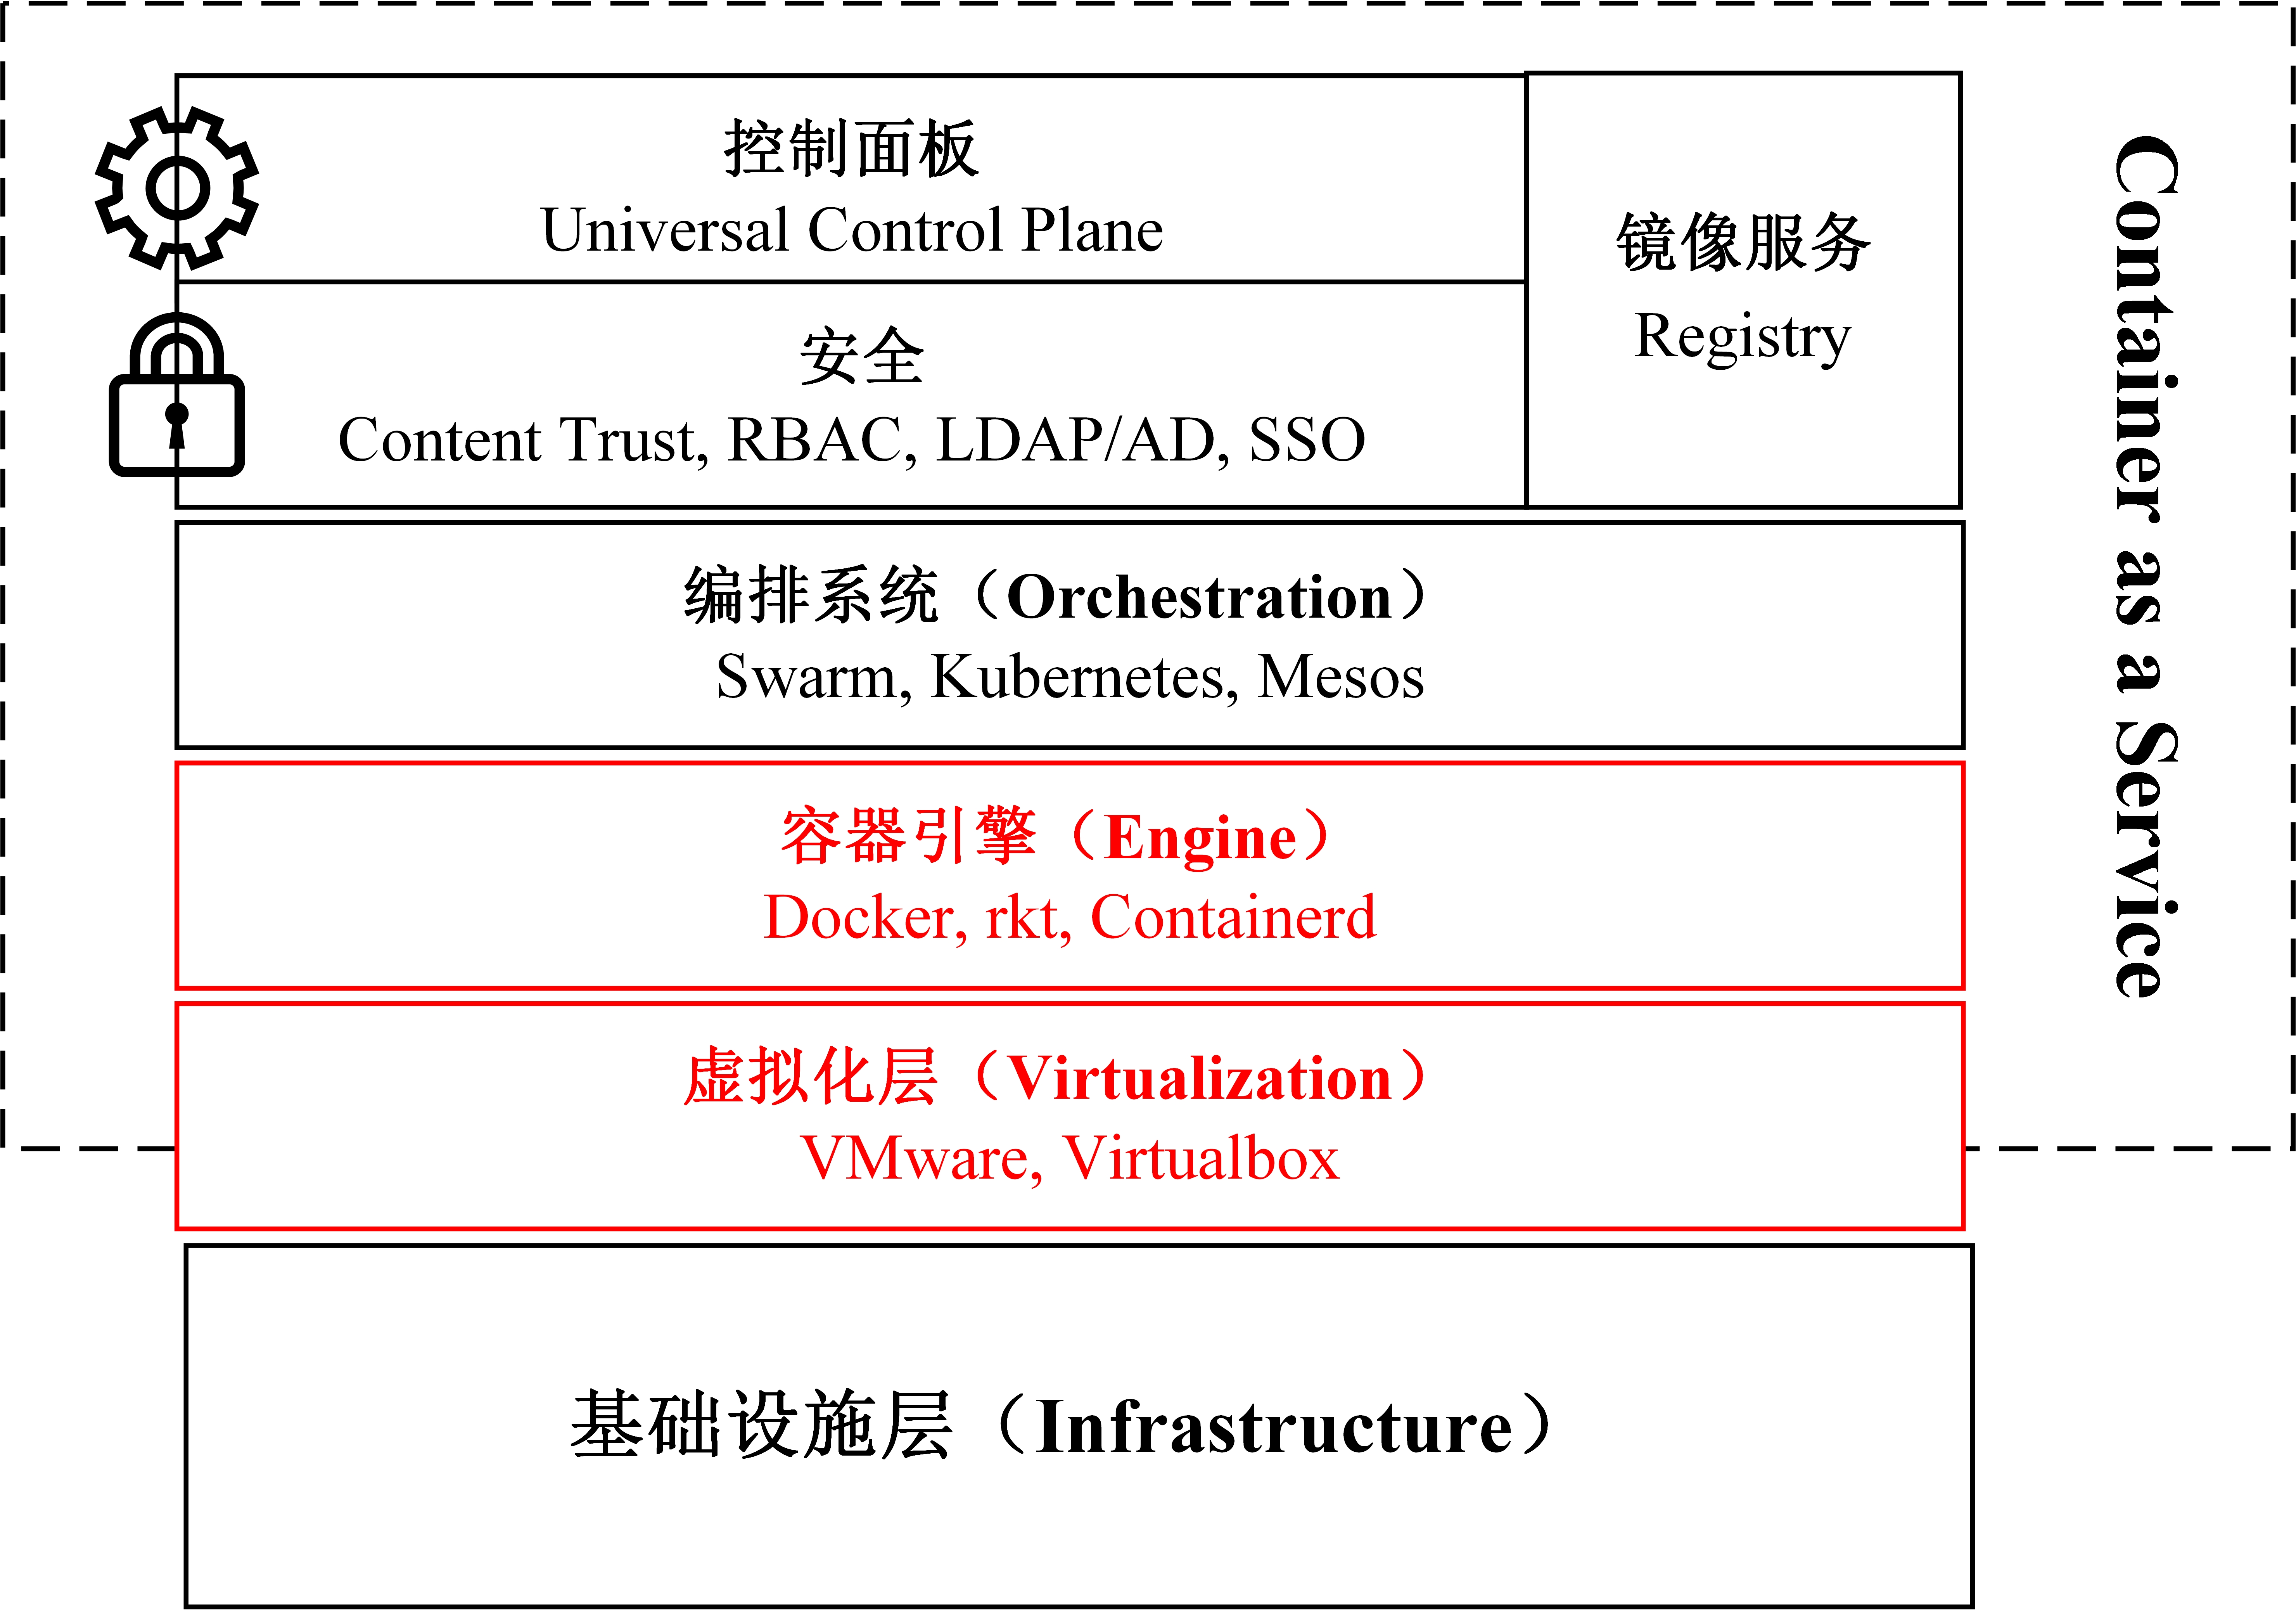
\includegraphics[scale=0.3]{figures/fig2_caas.jpg}
    \caption{CaaS架构示意图}
    \label{fig:fig2}
    \end{minipage}
}
\end{figure}

\end{frame}
